\newpage
\section{Introduction}
\label{sec:introduction}
\vspace{4.5mm}
% state the learning objective
\par In this laboratory assignment, an AC/DC converter was built, using a transformer and components such as diodes, resistors and capacitors. It is obvious to think that every component has its cost. Hence, the process of choosing what to use must be in line with the most accuracy possible, while keeping a reasonable price.
\vspace{3mm}
\par It was considered an input AC voltage with amplitude $230$V and frequency $50$Hz, aiming to a DC output of $12$V. The merit (M) measures the relation accuracy/cost and it is calculated with

\begin{equation}
M=\frac{1}{cost*(ripple(v_O)+average(v_O-12)+10^{-6}}
\end{equation}

with $v_O$ being the output DC voltage.
The considered circuit is presented in Figure ~\ref{fig:rc}.
\vspace{3mm}

\begin{figure}[h] \centering
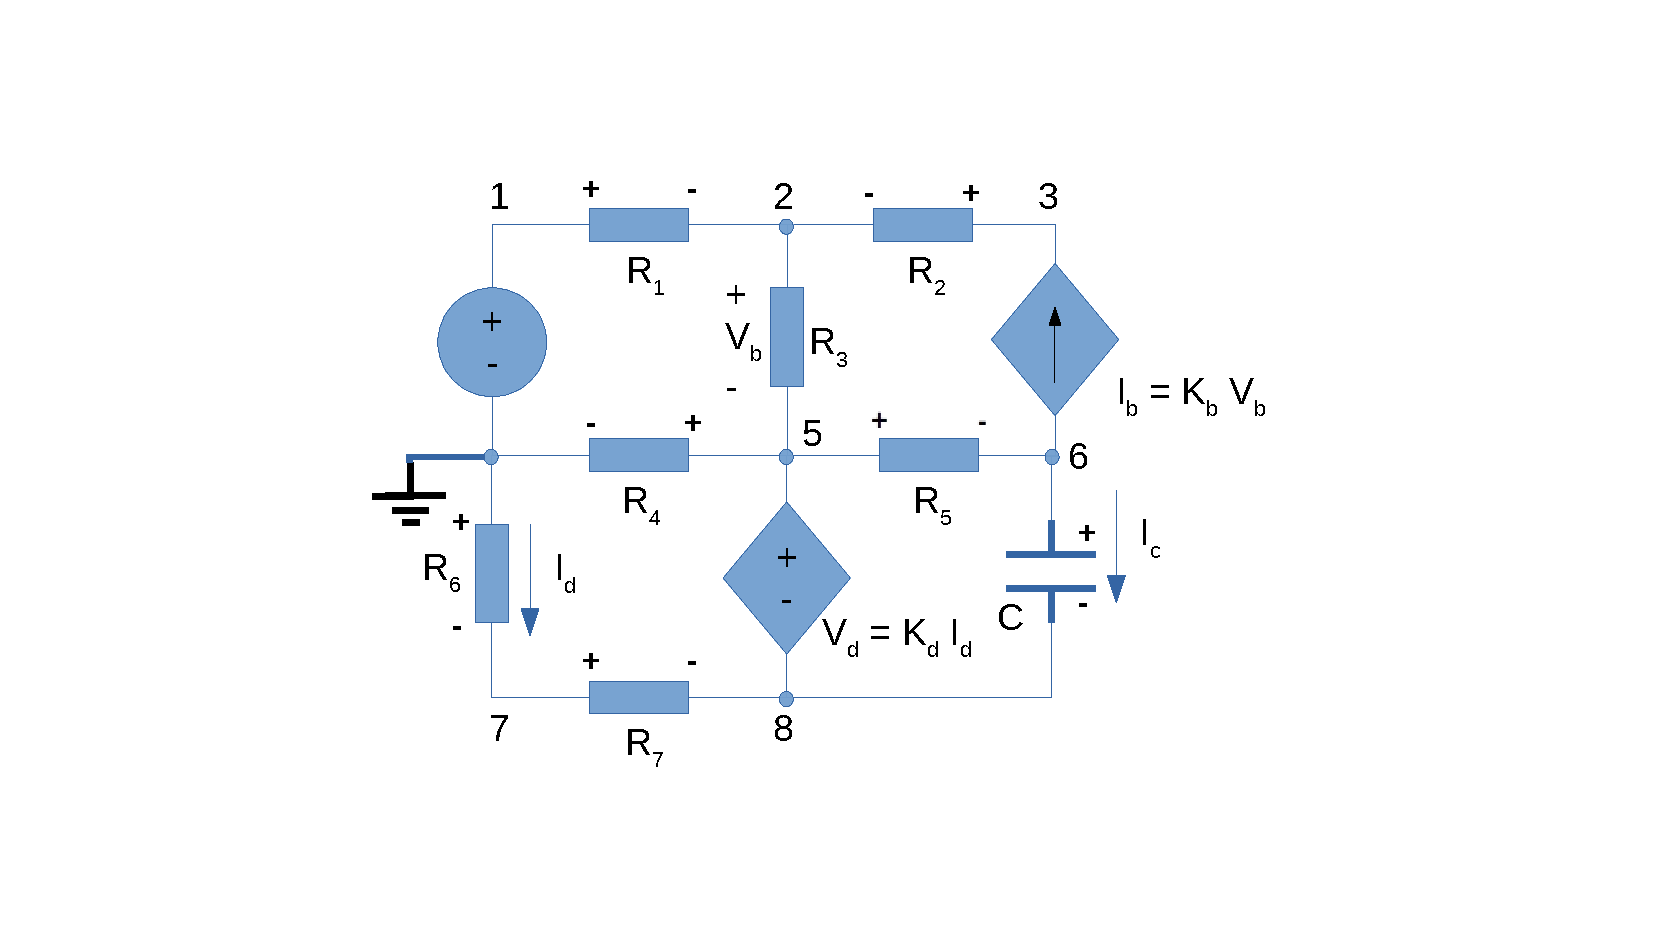
\includegraphics[scale=0.5]{rc.pdf}
\caption{AC/DC Converter considered.}
\label{fig:rc}
\end{figure}

\par In Section~\ref{sec:analysis}, a theoretical analysis of the circuit is presented, using Circuit Theory and Electronics Fundamentals concepts. After that, in Section~\ref{sec:simulation}, the circuit is analysed via simulation, using the software Ngspice. The obtained results are then compared, explaining the reasons behind the differences and similarities found. Finally, one can find the conclusions of this study outlined in Section~\ref{sec:conclusion}.
